%************************************************
\chapter{Definitions}
\label{ch:toolbox}
%************************************************

{\sffamily\slshape The text in this chapter is identical to Section 2 of the published version of the preprint at \href{https://arxiv.org/abs/2411.15900}{arXiv:2411.15900} along with the figures.\\}

In this chapter, the mathematical models for chemical reaction networks and pathways in them are presented,
namely directed hypergraphs and integer hyperflows, respectively.
This section is based on previous work which have used these concepts \cite{jakob_reactions_hypergraph,jakob_integer_hyperflows}. 

%%%%%%%%%%%%%%%%%%%%%%%%%%%%%%%%%%%%%%%%%%%%%%%%%%%%%%%%%%%%%%%%%%%%%%%%%%
\section{Directed Hypergraphs}
\label{sec:hypergraphs}
%%%%%%%%%%%%%%%%%%%%%%%%%%%%%%%%%%%%%%%%%%%%%%%%%%%%%%%%%%%%%%%%%%%%%%%%%%

A chemical reaction network consists of set of molecules $V$ and a set of reactions $E$.
Each reaction $e\in E$ is generally a many-to-many mapping of molecules,
which can be written~\cite{christoph_reaction_network_chemical} as the formal sum
\begin{equation*}
        e \colon \sum_{v\in V} s_{ve}^{-} v \longrightarrow \sum_{v\in V} s_{ve}^{+} v 
        \label{chemical_equation}
\end{equation*}
where $s_{ve}^{-}$ and $s_{ve}^{+}$ denote the stoichiometric coefficients,\\
\begin{tabular}{ll}
$s_{ve}^{-}$ & is the number of molecules of $v$ that are used \\
$s_{ve}^{+}$ & is the number of molecules of $v$ that are produced \\
\end{tabular}

\noindent by reaction~$e$.
\footnote{Note that the use of $^+$ and $^-$ is swapped compared to the notation in the referred previous work using hyperflows~\cite{jakob_integer_hyperflows}).}
The sum is over the entire set of molecules $V$ in the chemical reaction network,
and for molecules $v$ that do not take part in a particular reaction $e$, we have $s^-_{ve} = s^+_{ve} = 0$

A chemical reaction network is formally well represented~\cite{jakob_integer_hyperflows} as a directed multi-hypergraph~$(V, E)$, where

\begin{tabular}{l}
the set~$V$ of vertices models molecules and \\
the set~$E$ of directed multi-hyperedges models reactions. \\
\end{tabular}

A directed multi-hyperedge $e\in E$ is an ordered pair $(e^-, e^+)$ of multisets of vertices, which represents a reaction in the chemical reaction network.
The elements of $e^-$ model the reactants of the reaction, with each reactant $v$ appearing $s^-_{ve}$ times,
and correspondingly $e^+$ and $s^+_{ve}$ model the products of the reaction. An example hyperedge representing a chemical reaction is shown in Figure~\ref{fig: hyperedge}.
\newpage

\begin{figure}[!t]
	\centering
	\vspace{0.5cm}
    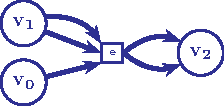
\includegraphics[scale=1.5]{graphics/chapter0/hyperedge.pdf}
    \vspace{0.5cm}
    \caption{A directed hyperedge, which represents a reaction where one copy of the molecule represented by the vertex $v_0$ reacts with two copies of $v_1$ to produce two copies of $v_2$. 
    This hyperedge can be considered to represent the reaction with the vertices representing the molecules: $v_0 \equiv$ O$_2$, $v_1 \equiv$ H$_2$ and $v_2 \equiv$ H$_2$O and the directed hyperedge representing the chemical reaction $e :$ O$_2$ + 2 H$_2$ $\longrightarrow$ 2 H$_2$O.}
    \label{fig: hyperedge}
\end{figure}

\begin{figure}[!ht]
    \centering
    \vspace{1cm}
    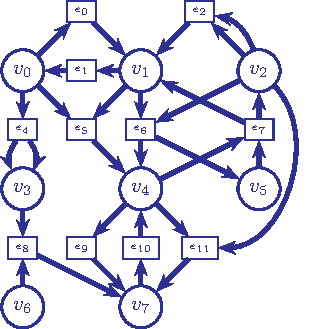
\includegraphics[scale=1.5]{graphics/chapter0/hypergraph.pdf}
    \vspace{0.4cm}
    \caption{A directed hypergraph, where circles are vertices and the squares are hyperedges.
    Hyperedges with multiple copies of a vertex as source or target are depicted with parallel arrows.
    See for instance~$e_4$, which has $v_3$ twice as a target and thus represents the reaction $e_4 : v_0 \rightarrow 2 v_3$. Hyperedges allow the many-to-many relations in chemical reaction to be captured in themodelling unlike edges in simple directed graphs.}
    \label{fig: hypergraph}
\end{figure}

\newpage

Figure~\ref{fig: hypergraph} depicts a hypergraph with eight vertices and eleven hyperedges.
As examples, \\
\begin{tabular}{ll}
	hyperedge~$e_0$ &$\equiv (\{v_0\}, \{v_1\})$ \\
	& represents the one-to-one reaction $v_0\rightarrow v_1$, \\
	hyperedge~$e_3$ &$\equiv (\{v_0, v_1\}, \{v_3\})$  \\
	& represents the many-to-one reaction \\
	& $v_0 + v_1\rightarrow v_3$, \\
	hyperedge~$e_2$ &$\equiv (\{v_2, v_2\}, \{v_1\})$ \\
	& represents the many-to-one reaction $2 v_2\rightarrow v_1$, \\
	hyperedge~$e_4$ &$\equiv (\{v_3\}, \{v_0, v_1\})$ \\
	& represent the one-to-many reaction \\
	& $v_3\rightarrow v_0 + v_1$, \\
	hyperedge~$e_7$ &$\equiv (\{v_3\}, \{v_5, v_5\})$ \\
	& represent the one-to-many reaction \\
	& $v_3\rightarrow 2 v_5$, and \\
	hyperedge~$e_9$ & $\equiv (\{v_3, v_4\}, \{v_7, v_8\})$ \\
	& represents the many-to-many reaction \\
	& $v_3 + v_4\rightarrow v_7 + v_8$.\\
\end{tabular}

On a related note, standard usage of the term `reaction' implies the breaking and forming of chemical bonds.
However, physical processes that do not alter the set of bonds in a molecule yet involve energy transformations, thereby affecting the molecule's ability to participate in a reaction.
For instance, some reactions occur only when a molecule is excited into a higher energy state, or certain molecules (such as phosphorus or sulfur) are in specific phases.
Although such transitions are not conventionally termed `reactions,' they are elementary processes accompanied by a change in free energy.
Consequently, in the rest of this paper we will use the term `reaction' to denote this broader set of relations between classes of molecules. 

%%%%%%%%%%%%%%%%%%%%%%%%%%%%%%%%%%%%%%%%%%%%%%%%%%%%%%%%%%%%%%%%%%%%%%%%%%
\section{Integer Hyperflows}
\label{sec:hyperflows}
%%%%%%%%%%%%%%%%%%%%%%%%%%%%%%%%%%%%%%%%%%%%%%%%%%%%%%%%%%%%%%%%%%%%%%%%%%
A pathway is a set of reactions that transforms some available source molecules into desired target molecules.
To model pathways formally, the concept of an \emph{integer hyperflow}~$f$ in a hypergraph~$\mathcal{H} = (V,E)$ was introduced by~\cite{jakob_integer_hyperflows}.

A pathway is viewed as a vector $f_E \in \mathbb{N}_{0}^{|E|}$,
i.e., an assignment of a non-negative integer to each edge in~$E$, denoting how many times the corresponding reaction appears in the pathway.
Additionally, two vectors $f_{\text{in}} \in \mathbb{N}_{0}^{|V|}$ and $f_{\text{out}} \in \mathbb{N}_{0}^{|V|}$ denote for each molecule in~$V$ the amount of it consumed as source molecule, respectively produced as target molecule, by the pathway.

\begin{figure}[!t]
    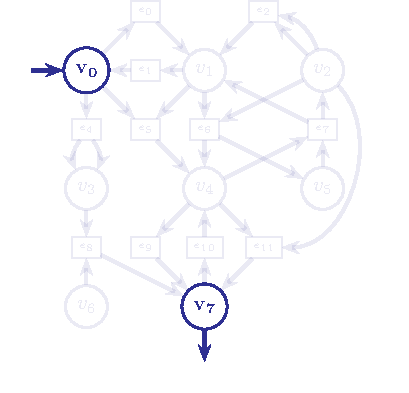
\includegraphics[scale=1.5]{graphics/chapter0/flowQuery.pdf}
    \vspace{0.5cm}
    \caption{An integer hyperflow query in the directed hypergraph from Figure~{ref: hypergraph}, where $v_0$ is specified as the source and $v_7$ is specified as the target. 
    The exact inflow and outflow on these vertices are not specified, and the hyperpaths in Figure~\ref{fig: hyperpath1}, \ref{fig: hyperpath2}, \ref{fig: hyperpath3}, \ref{fig: hyperpath4} and \ref{fig: hyperpath5} would be valid solutions of this flow query if the required additional sets of vertices is allowed as sources (which are {\O}, $\{v_2\}$, $\{v_1\}$, $\{v_2\}$, $\{v_6\}$ respectively).
    If additional vertices are not allowed as sources, only the hyperpath in Figure~\ref{fig: hyperpath1} is a valid solution.}
    \label{fig: flow_query}
\end{figure}


The pathway's net effect on the number of molecules in the system is specified entirely by $f_{\text{in}}$ and $f_{\text{out}}$.
\begin{equation}
    \mathbf{S}^+\cdot f_E  - \mathbf{S}^-\cdot f_E =  f_{\text{out}} - f_{\text{in}}
    \label{int_hyperflow_matrix}
\end{equation}
where

\begin{tabular}{ll}
$\mathbf{S}^-$ & is a $|V|\times |E|$ matrix with entries~$s_{ve}^-$ \\
$\mathbf{S}^+$ & ia a $|V|\times |E|$ matrix with entries~$s_{ve}^+$ \\
\end{tabular}

\noindent (recall from definition of hypergraphs that $s_{ve}^-$ and $s_{ve}^+$ are the numbers of molecule $v$ consumed and produced by reaction $e$).
In hypergraph terminology, $\mathbf{S}^-$ and $\mathbf{S}^+$ are the out-incidence matrix and the in-incidence matrix, respectively.% dont remove this comment, it escapes the newline
\footnote{
    In other settings, $\mathbf{S}^-$ and $\mathbf{S}^+$ are called the reactant stoichiometric matrix and the product stoichiometric matrix.
    One can also meet a single stoichiometric matrix, defined as $\mathbf{S} = \mathbf{S}^+ - \mathbf{S}^-$.
    This latter version is less expressive for chemical reaction network modeling, as the role of catalysts and autocatalytic molecules cannot be captured.
    In some contexts, $f_{\text{in}}$ and $f_{\text{out}}$ are called the external compounds.
}
The matrices $\mathbf{S}^-$ and $\mathbf{S}^+$ for the hypergraph in Figure \ref{fig: hypergraph} are shown in Figure \ref{fig: stoichoimetric_matrix}.

\begin{figure}[!t]
	\centering
	\begin{subfigure}{0.75\textwidth}
		\begin{small}
		\[       
		    \kbordermatrix{
		            &e_0&e_1&e_2&e_3&e_4&e_5&e_6&e_7&e_8&e_9&e_{10}\\
		        v_0 & 1 &   &   & 1 &   &   &   &   &   &   &   \\
		        v_1 &   & 1 &   &   &   & 1 &   &   &   &   &   \\
		        v_2 &   &   & 2 &   &   & 1 &   &   &   &   & 1 \\
		        v_3 &   &   &   &   & 1 &   &   & 1 &   &   &   \\
		        v_4 &   &   &   &   &   &   & 1 &   &   & 1 & 1 \\
		        v_5 &   &   &   &   &   &   &   &   &   &   &   \\
		        v_6 &   &   &   &   &   &   &   &   &   &   &   \\
		        v_7 &   &   &   &   &   &   &   &   &   &   &   \\
		        v_8 &   &   &   &   &   &   &   &   &   &   &  
		    }
		\]
		\end{small}
		\caption{in-incidence matrix}
		\label{in_incidence}
    \end{subfigure}
    \\
    \vspace{0.5cm}
    \begin{subfigure}{0.75\textwidth}
    	\begin{small}
		\[
		    \kbordermatrix{
		            &e_0&e_1&e_2&e_3&e_4&e_5&e_6&e_7&e_8&e_9&e_{10}\\
		        v_0 &   & 1 &   &   & 1 &   &   &   &   &   &   \\
		        v_1 & 1 &   & 1 &   &   &   & 1 &   &   &   &   \\
		        v_2 &   &   &   &   &   &   & 1 &   &   &   &   \\
		        v_3 &   &   &   & 1 &   &   &   &   &   &   &   \\
		        v_4 &   &   &   &   &   & 1 &   &   &   &   &   \\
		        v_5 &   &   &   &   &   &   &   & 2 &   &   &   \\
		        v_6 &   &   &   &   &   &   &   &   & 1 &   & 1 \\
		        v_7 &   &   &   &   &   &   &   &   &   & 1 &   \\
		        v_8 &   &   &   &   &   &   &   &   &   & 1 & 
		    }
		\]
		\end{small}		
		\caption{in\\out-incidence matrix}
		\label{out_incidence}
	\end{subfigure}
    \caption{A representation of the hypergraph from Figure \ref{fig: hypergraph} as \ref{out_incidence} an out-incidence matrix $\mathbf{S}^-$ and \ref{in_incidence} an in-incidence matrix $\mathbf{S}^+$.
    Only non-zero entries are shown.
    Since the hypergraph has $9$ vertices and $11$ hyperedges, the matrices have dimensions $9 \times 11$.}
    \label{fig: stoichoimetric_matrix}
\end{figure}

To unify the three vectors~$f_E$, $f_{\text{in}}$, and $f_{\text{out}}$ into a single flow vector on hyperedges,
\cite{jakob_integer_hyperflows} introduced for each $v \in V$ two so-called half-edges

\begin{tabular}{l}
$e_v^+ = (\emptyset, v)$ and \\
$e_v^- = (v, \emptyset)$ \\
\end{tabular}

\noindent These represent the production of~$v$ as source molecule addition to the system and the consumption of~$v$ as target molecule removal from the system, respectively.
Setting
$$
\begin{array}{lcl}
E^+ & = & \{ e_v^+ \mid  v \in V\}\\
E^- & = & \{ e_v^- \mid  v \in V\}\\
\overline{E} & = & E \cup E^+ \cup E^-,\\
\end{array}
$$
\cite{jakob_integer_hyperflows} introduced the extended hypergraph $\overline{\mathcal{H}} = (V, \overline{E})$
and defined an \emph{integer hyperflow} to be a vector $f \in \mathbb{N}_{0}^{|\overline{E}|}$ satisfying the flow conservation constraint
\footnote{A detailed discussion of how integer hyperflows relate to, and differ from, other similar concepts such as elementary modes, extreme pathways, and flux balance analysis can be found in Section 2.6 of~\cite{jakob_integer_hyperflows}.}
\begin{equation}
    \forall v\in V\colon \sum_{ e\in \overline{E} } s_{ve}^+ f_e - \sum_{ e\in \overline{E} } s_{ve}^- f_e = 0 
    \label{int_hyperflow_jakob}
\end{equation}
where,

\begin{tabular}{ll}
$s_{ve}^-$ & an entry in the $|V|\times |\overline{E}|$ out-incidence matrix of $\overline{\mathcal{H}}$ \\
$s_{ve}^+$ & an entry in the $|V|\times |\overline{E}|$ in-incidence matrix of $\overline{\mathcal{H}}$ \\
$f_e$ & an entry in $f$ \\
\end{tabular}

\newpage
\begin{figure}[!ht]
    \centering
    \begin{subfigure}{0.48\textwidth}
        \centering
        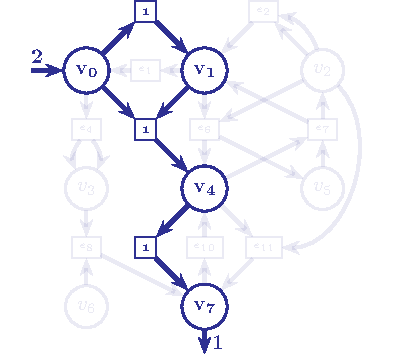
\includegraphics[width=\textwidth]{graphics/chapter0/hyperpath1.pdf}
        \caption{hyperpath 1}
        \label{fig: hyperpath1}
    \end{subfigure}%
    \hfill
    \begin{subfigure}{0.48\textwidth}
        \centering
        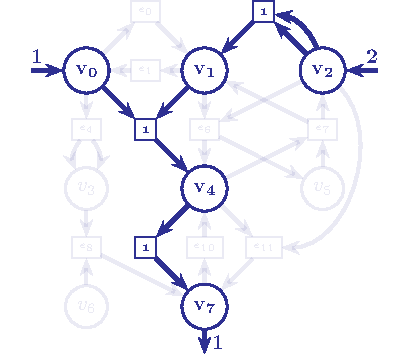
\includegraphics[width=\textwidth]{graphics/chapter0/hyperpath2.pdf}
        \caption{hyperpath 2}
        \label{fig: hyperpath2}
    \end{subfigure}
    \\
    \vspace{0.5cm}
    \begin{subfigure}{0.48\textwidth}
        \centering
        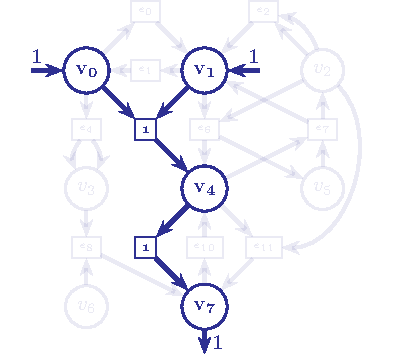
\includegraphics[width=\textwidth]{graphics/chapter0/hyperpath3.pdf}
        \caption{hyperpath 3}
        \label{fig: hyperpath3}
    \end{subfigure}%
    \hfill
    \begin{subfigure}{0.48\textwidth}
        \centering
        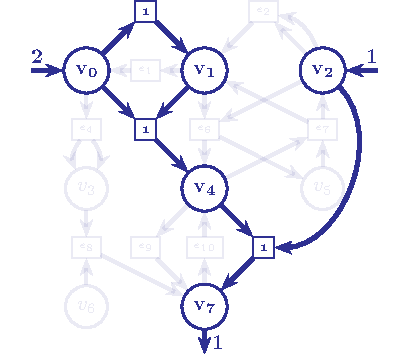
\includegraphics[width=\textwidth]{graphics/chapter0/hyperpath4.pdf}
        \caption{hyperpath 4}
        \label{fig: hyperpath4}
    \end{subfigure}
    \\
    \vspace{0.5cm}
    \begin{subfigure}{0.48\textwidth}
        \centering
        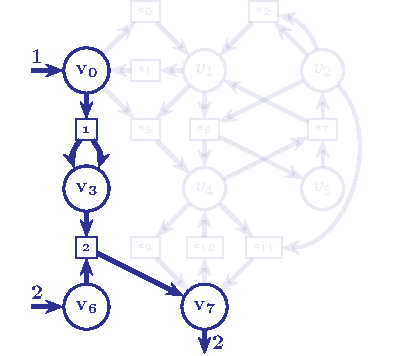
\includegraphics[width=\textwidth]{graphics/chapter0/hyperpath5.pdf}
        \caption{hyperpath 5}
        \label{fig: hyperpath5}
    \end{subfigure}%
    \hfill
    \begin{subfigure}{0.48\textwidth}
        \centering
        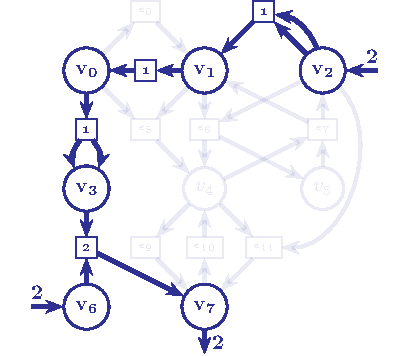
\includegraphics[width=\textwidth]{graphics/chapter0/hyperpath6.pdf}
        \caption{hyperpath 6}
        \label{fig: hyperpath6}
    \end{subfigure}
    \vspace{0.4cm}
    \caption{Six possible integer hyperflows \ref{fig: hyperpath1}, \ref{fig: hyperpath2}, \ref{fig: hyperpath3}, \ref{fig: hyperpath4}, \ref{fig: hyperpath5}, and \ref{fig: hyperpath6} in the hypergraph from Figure \ref{fig: hypergraph}, each representing a pathway,
    where hyperedges with non-zero flow are drawn in bold. The integers in the boxes represent the hyperflow assigned to the respective hyperedge in the pathway.}
    \label{fig: hyperflow}
\end{figure}

\newpage
\noindent The constraint in Equation~\eqref{int_hyperflow_jakob} is easily seen to be equivalent to the constraint in Equation~\eqref{int_hyperflow_matrix}. 

In Figure~\ref{fig: hyperflow}, six possible hyperflows in a hypergraph are depicted.
Unboxed integers are flow values on half-edges, while boxed integers are the flow values for hyperedges in $E$.
The inflow and the outflow are depicted as half-edges in and out of the source and target vertices of the pathway.
For clarity, only half-edges with non-zero flow values are shown.

One key feature of integer hyperflows is that they give a flexible and generic way to \emph{specify} pathways via constraints on the flow on half-edges.
This may be as straight-forward as specifying an overall reaction for the pathway by fixing the flow on the half-edges for the molecules in the source and target sets and setting the flow to zero for the rest of the half-edges.
Or one may specify upper and lower limits for some half-edges and free values for others,
for instance to ask if there is any way to produce at least some target molecules using any amount of source molecules,
while at the same time allowing waste products.

Then a \emph{search} for pathways fulfilling the specification amounts to finding flow vectors~$f$ obeying those constraints, in addition to the constraint in Equation~\eqref{int_hyperflow_jakob}.
Since integer hyperflows are integer valued, it is natural to model the situation via the ILP formalism and search for~$f$ using an ILP solver.
This idea has been implemented as part of the software system~MØD~\cite{mod_web}.
The result is a powerful and flexible tool for specifying and searching for pathways (integer hyperflows) in a given chemical reaction network (hypergraph).
The flexibility is further increased by the possibility of having flow values in the ILP objective function, such that e.g.\ flow solutions allowing but minimizing waste can be found.
Also the flow values on non-half-edges can enter the specification and/or optimization,
allowing e.g.\ the search for solutions minimizing the use of a given reaction deemed particularly expensive to include in the pathway.

\section{Hyperflows and Fluxes}
\label{sec: comparison}

In this section, we give a comparison of our workflow with existing methods. Constraint-based models such as flux balance analysis also use constraint programming with an objective function that is optimized. For instance, open-source tools such as COBRApy~\cite{cobrapy} perform flux analysis on a reaction network supplied to them. However, such tools do not construct the network on the fly in a generative way--- rather the reaction network has to be constructed beforehand using some other tool. Flux balance analysis generates a flux vector for the reactions in the network which is allowed to contain floating-point values, while our method accepts only integers as a valid hyperflow for a reaction, which is more aligned with the standard notion of a pathway. Formulating a flux balance analysis on the network would be equivalent to an LP relaxation of the pathway query problem using integer hyperflows for the same network. A linear program (LP) can be solved in polynomial time while an ILP is NP-hard. However, formulating the search for pathways to a queried molecule in a reaction network offers some advantages.

\begin{figure}
    \centering
    \begin{subfigure}{\textwidth}
        \centering
        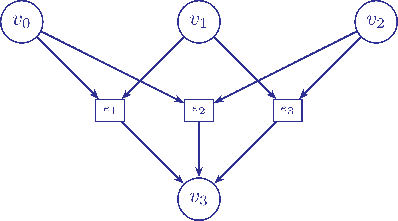
\includegraphics[scale=1.0]{graphics/chapter0/example_network.pdf}
        \vspace{0.4cm}
        \caption{An example reaction network with $4$ molecules and $3$ reactions.}
        \label{fig:example_network}
    \end{subfigure}\\
    \vspace{0.8cm}
    \begin{subfigure}{\textwidth}
        \centering
        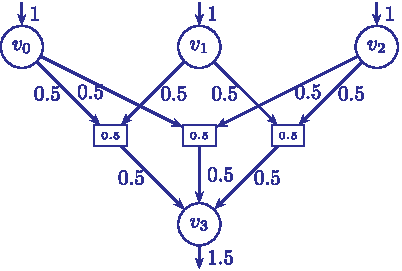
\includegraphics[scale=1.0]{graphics/chapter0/example_flux.pdf}
        \vspace{0.4cm}
        \caption{A flux distribution in the network which produces an outflow of $1.5$ for $v_3$.}
        \label{fig:example_flux}
    \end{subfigure}\\
    \vspace{0.8cm}
    \begin{subfigure}{\textwidth}
        \centering
        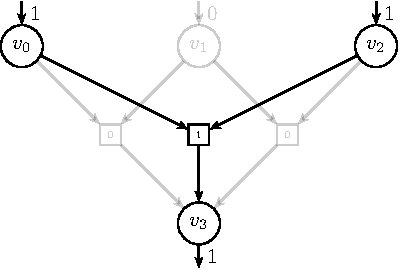
\includegraphics[scale=1.0]{graphics/chapter0/example_flow.pdf}
        \vspace{0.4cm}
        \caption{An assignment of integer hyperflows in the network which produces an outflow of $1$ for $v_3$.}
        \label{fig:example_flow}
    \end{subfigure}
    \vspace{1cm}
    \caption{Comparison of flux balance analysis and an integer hyperflow in an example reaction network.}
    \label{fig:comparison}
\end{figure}

There exists reaction networks where the optimal solutions from the ILP formulated by our modeling and the relaxed LP from flux balance analysis differ. Consider the reaction network shown in Figure~\ref{fig:example_network} with the following formulation of the problem:
\begin{align*}
    &\max \left( \text{outflow}(v_3) \right) \\
    \text{subject to: } &\text{inflow}(v_0) + \text{inflow}(v_1) +\text{inflow}(v_2) \leq 3
\end{align*}
The optimal flux distribution yields an objective value of $1.5$ with the assigned fluxes shown in Figure~\ref{fig:example_flux} while our method assigns the integer hyperflows shown in Figure~\ref{fig:example_flow} in one of the three optimal solutions with objective value $1$. The other two solutions assign the hyperflows $(0,1,1)$ and $(1,1,0)$ to the hyperedge set $(e_1,e_2,e_3)$ respectively.

The ILP solution space is a subset of the LP feasible reaction and therefore, the objective value for the optimal solution for the relaxed LP will always be as at least as large as the objective value of optimal solution for the corresponding ILP. This is illustrated in the example shown in Figure~\ref{fig:comparison} too. As the result, the fluxes and the structure of the solution is often different from those if they were constrained to be integers.

Restricting hyperflows to integers makes physical sense because molecules occur and react in discrete quantities.
Actually, small molecular counts in several biological settings (often involving trace amounts of enzymes and inhibitors affecting multiple iterations of the same pathway) and physical cases (as in chain reactions and cascades) do not allow arbitrary scaling of the number of molecules, as the use of real-valued fluxes by flux balance analysis assume.
When a small number of molecules are encountered in a scenario as above (or in scenarios with appearances of a rare but significant molecule in the system), the discrete nature of the molecules becomes more pronounced.

Another feature of our proposed method is the enumeration of alternative pathways with disjoint set of hyperedges ranked on the basis of a chosen objective function. While flux balance analysis offers the possibility to find alternative pathways~\cite{fba_alternative_pathways}, they have the same objective value but a different flux distribution in the network. This differs from the enumeration of solutions in the current method which offers a list of pathways ordered by the increasing value of the objective function for the user to choose from. Enumerating solutions over variables with a continuous domain is difficult using indicator variables and biimplications as in constraints \ref{biimp1}  and \ref{biimp2}. The enumeration of solutions offers diverse pathways to the queried molecules and makes the method more robust to uncertainties in the weights assigned to the hyperedges.
